\documentclass[adobefonts,a4paper]{ctexart}

\usepackage[top=1.2in, bottom=1.2in, left=1in, right=1in]{geometry}
\usepackage{fancyvrb,graphicx,hyperref}

\hypersetup{
colorlinks=true,
linkcolor=blue
}

%opening
\title{实验报告}
\author{计科一班\quad蔡日骏\quad12348003}
\date{\today}

\renewcommand{\textfraction}{0.15}
\renewcommand{\topfraction}{0.85}
\renewcommand{\bottomfraction}{0.65}
\renewcommand{\floatpagefraction}{0.60}

\begin{document}

\maketitle
\section{概述}
本作品根据作业要求第四种方案完成。\footnote{类层次稍有不同,详情请看\ref{design}节}
程序提供GUI,使用Qt实现,可在Qt 4.8及Qt 5.0下编译。由于使用部分C++ 11特性,需要在
g++ 4.7或以上版本中编译。

\SaveVerb{doxygen}|./report/doxygen/index.html|
代码的详细结构在可在实验报告附带的doxygen文档\footnote{\UseVerb{doxygen}文件中。}中查看。

\section{设计过程及讨论}
\subsection{设计思路}\label{design}

\SaveVerb{Student}|Student|

由于程序逻辑比较复杂,为了便于描述和开发,使用MVC架构的设计。各层设计及对应的类如下。
\emph{(所有类封装在\UseVerb{Student}命名空间中。)}

\begin{itemize}
 \item Model层
 负责管理数据,以及对数据的直接操作。
 
 首先,使用一个 \verb|Student|类保存一个学生的个人信息。这个类只提供只读接口,因为对下面将要提到的
 \verb|StudentBase|类来说,``添加学生''和``修改学生''操作的接口被统一为一个以简化程序,因此对
 学生信息的修改可以通过直接替换 \verb|Student|对象来完成。\verb|Student|类的UML图如图 \ref{fig:uml_student}。
 
 \begin{figure}[htbp]
  \centering
  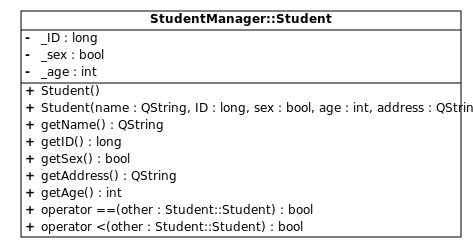
\includegraphics[scale=0.8]{Student}
  \caption{\protect\UseVerb{Student}类UML} \label{fig:uml_student}
 \end{figure}

 然后,定义一个 \verb|StudentBase|类作为处理招生办数据的模型层。这个类负责读取和写入数据,提供查询和写入学生基本信息的
 接口,同时提供 \verb|loadStudentList|以及 \verb|loadAStudentDetails|模板函数方便上层加载数据。这两个模板函数接受
 一个``操作''\footnote{函数指针、函数对象或$\lambda$表达式,``操作''指实际进行数据加载的``操作''。}
 作为参数,可以认为两个函数为高阶函数。
 
 由于三个系的类需要提供相同的接口,功能也基本相同,因此为所有系的类定义一个接口 \verb|IFaculty|,实现了各系类的功能,而各
 系类只需要继承 \verb|IFaculty|类,并使用相应的设置\footnote{最少主修课程、最少辅修课程、文件名等。}对
 \verb|IFaculty|类进行初始化即可。由于只需要保存一份学生基本信息,而这里的继承基本上仅限于数据层面上而不是公开接口上,
 因此,\verb|IFaculty|对 \verb|StudentBase|进行\verb|virtual protected|继承。
 
 三个系的类 \verb|FacultyA|、\verb|FacultyB|、\verb|FacultyC|,继承\verb|IFaculty|类,并用不同的初始化参数对
 \verb|IFaculty|类进行初始化。由于每个专业需要保存自己的一份成绩,因此不使用虚继承,只进行公有继承。
 
 学位办的 \verb|StudentMIS|类保护继承 \verb|FacultyA|、\verb|FacultyB|、\verb|FacultyC|类,提供所有信息的查询及
 数据统计功能。由于不需要写入功能,\verb|StudentMIS|类不提供写入的接口。
 
 Model层各类继承关系如图 \ref{fig:uml_model}。
 
 \begin{figure}[htbp]
  \centering
  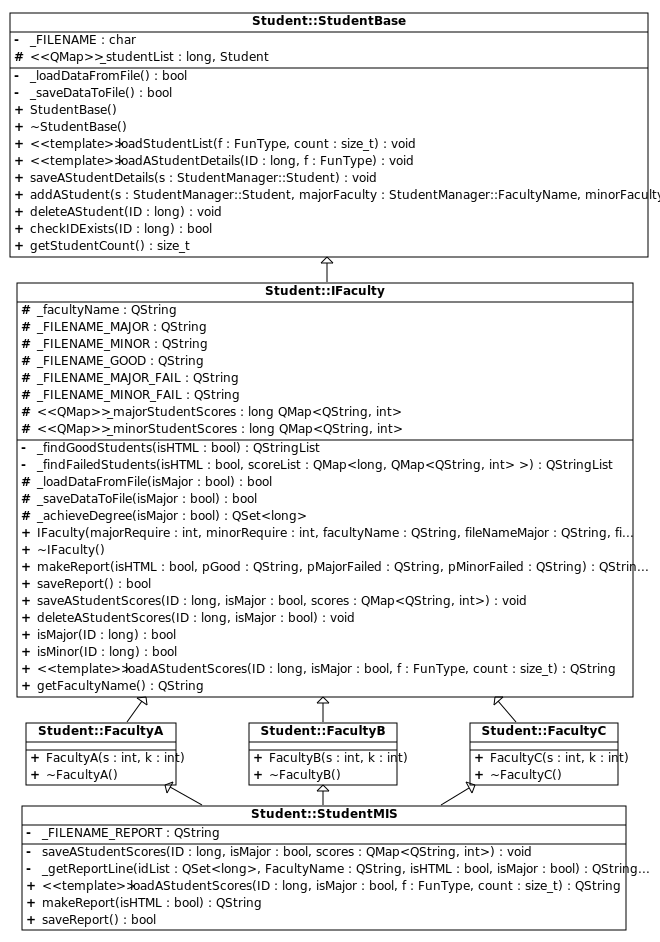
\includegraphics[scale=0.8]{Model}
  \caption{Model层类UML} \label{fig:uml_model}
 \end{figure}
 
 
 \item Controller层
 
 \SaveVerb{_ui}|IController::_ui|
 
 Controller层为提供统一接口,定义一个抽象类 \verb|IController|作为接口。 \verb|IController|类指定了Controller层
 类需要实现的接口。Controller层的类对象保存View层传递过来的 \verb|Ui::StudentMain|指针\footnote{\UseVerb{_ui}},
 用于Controller层对UI的操作。
 
 \verb|AdmissionsOfficeController|、\verb|FacultyController|、\verb|DegreesOfficeController|类分别对应
 招生办、系、学位办的登陆身份,对 \verb|IController|指定的接口进行实现。其中 \verb|FacultyController|可处理三个
 系的操作,因为三个系的Model层类均公开继承 \verb|IFaculty|。
 
 Controller层类的继承关系如图 \ref{fig:uml_controller}。
 
 \begin{figure}[htbp]
  \centering
  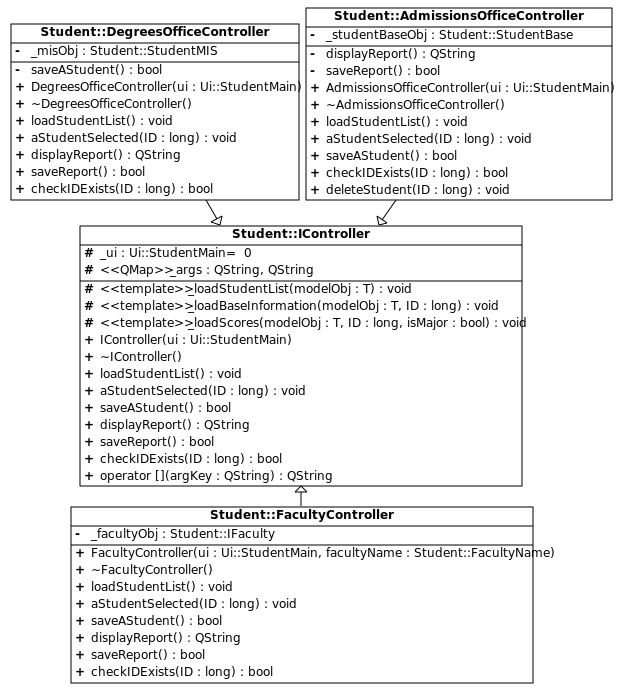
\includegraphics[scale=0.8]{Controller}
  \caption{Controller层类UML} \label{fig:uml_controller}
 \end{figure}
 
 
 \item View层
 
 View层主要为Qt自动生成的与GUI相关的几个类。其中比较重要的为 \verb|StudentMain.h|中定义的 \verb|StudentMain|类。
 该类负责响应GUI的事件,并通知Controller层进行处理。
 
 View层的 \verb|ui_XXX.h|、\verb|ui_XXX.cpp|文件在编译时由 \verb|qmake|自动生成。
\end{itemize}

\subsection{不足}
程序架构设计上最大的不足在于,为了尽可能满足题目中对类设计的要求,不得不把学生的基本信息与学生的成绩被分离开来,
造成某些操作的实现过于复杂。更合理的设计应该是由 \verb|Student|类以及 \verb|Student|类的派生类对象进行单个学生数据
的存储,然后Model层一个类使用容器保存多个 \verb|Student|类并提供相关操作,Controller层进行转发和访问控制。

另一个不足之处在于,由于数据存储格式限制,程序无法存储复杂的格式,如带空格的字符串。


\section{测试}
初始测试数据在程序目录下。程序运行时会自动加载。

以招生办身份登陆,点击学生列表下的``添加''按钮可添加学生。如果添加一个学号已存在的学生,程序将会报错。
填写学生学号、专业后,在右侧填写学生的基本信息,点击``保存'',即可成功添加学生。
点击``删除''按钮可以删除当前选中的学生。在右侧学生信息界面中,可以修改当前选中学生的基本信息,
但学号不允许修改。修改完成后点击``保存''即可保存修改。

以专业系身份登陆,选择学生后,可以查看学生的基本信息。如果该学生主修或辅修该专业系的课程,右下方的成绩框变成可用状态,
可以点击``添加''按钮添加课程成绩。填写好课程成绩后,点击``保存''即可保存修改。点击学生列表下的``统计''按钮,可以对
本专业系的学生成绩进行统计,并以统计报告的形式显示出来。在统计对话框中点击``保存''可按照题目要求保存统计结果。
如对专业A的数据进行统计,其结果如图 \ref{fig:FacAStat}。

\begin{figure}[htbp]
 \centering
 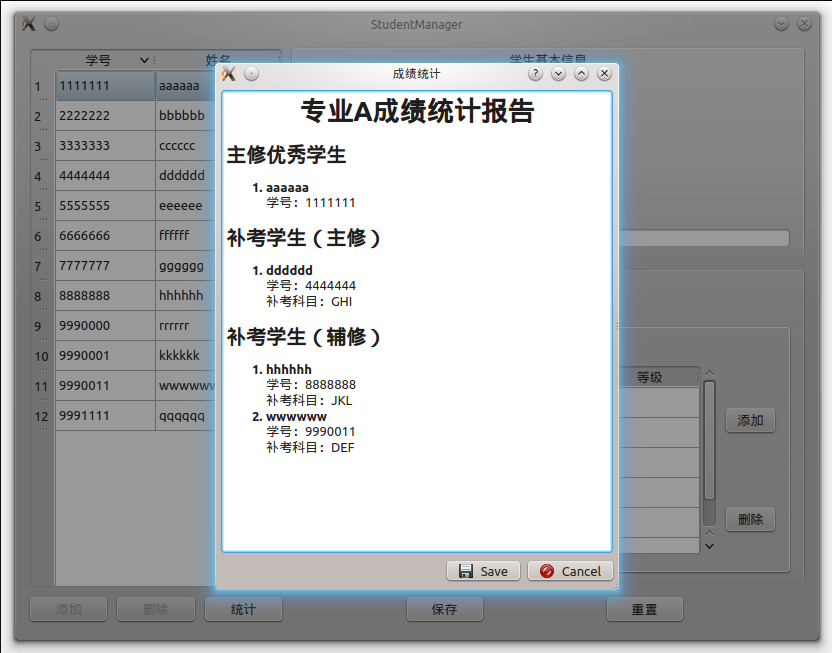
\includegraphics[scale=0.5]{FacAStat}
 \caption{对专业A数据进行统计} \label{fig:FacAStat}
\end{figure}

以学位办身份登陆,选择学生后,可以查看学生的所有信息。点击``统计''按钮,可以进行学位统计。统计结果如图 \ref{fig:DegStat}
点击统计对话框中的``保存''按钮可以按照题目要求保存统计结果。

\begin{figure}[htb!]
 \centering
 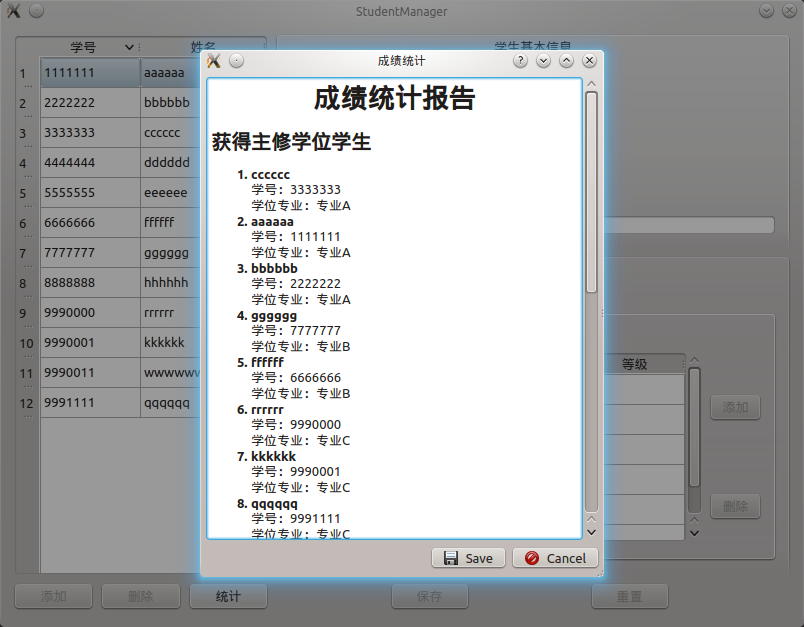
\includegraphics[scale=0.5]{DegStat}
 \caption{学位数据统计} \label{fig:DegStat}
\end{figure}

\section{小结}
这个实验作业主要难点在于逻辑比较复杂。实际上要粗糙地实现所有功能在理论上是可行的,但是会导致严重的代码冗余,也非常容易出错,
降低开发效率。而要优雅地实现这个程序,需要使用面向对象的思维对类进行认真设计。但是这样一来,有可能会导致为了解决代码冗余
而带来的开发复杂度大于代码冗余本身带来的复杂度。这需要去得一个平衡,找出适合这样一个规模的程序的类架构。

\end{document}
